Ce chapitre couvre la transmission des trames démodulées par le premier microcontrôleur vers le deuxième microcontrôleur. Dans la section suivante, le format des entrées et sorties de ce bloc vont être détaillées.\footnote{Ce chapitre couvre les fichiers \ilcode{uart.*} des projets \ilcode{communication.X} et \ilcode{propulsion.X}}

\section{Première analyse}
Puisqu'on désire limiter le nombre d'opérations effectuées par le microcontrôleur effectuant le traitement du signal audio, les trames de 10 bits renvoyées par la fonction \ilcode{fskDetector} sont envoyées telles quelles au deuxième microcontrôleur. L'entrée du bloc transmission est donc une trame de 10 bits. L'uart, implémenté en hardware des deux côtés est utilisé pour effectuer la transmission. Celui-ci utilise des trames de 8 ou 9 bits, et il faudra donc 2 trames d'UART pour transmettre une trame de FSK. L'émetteur et le récepteur sera donc logiquement des machines à état séquentielles. Plutôt que de simplement reconstituer la trame de 10 bits originale, on choisit que le récepteur renvoie directement d'une part les 2 bits de commande et d'autre part les 8 bits d'arguments contenus dans une transmission.

Les parties récepteur et émetteur vont être abordées en parallèle dans la suite, puisqu'elles sont fortement liées. Tout d'abord, la configuration des modules UART est examinée\footnote{La plupart des paramètres doivent forcément être les mêmes des deux côtés de la transmission pour que celle-ci soit possible.}, ensuite, l'émetteur et le récepteur vont être construits.

\section{Configuration des modules UART}
\subsection{Paramètres communs}
Pour que la communication soit possible, les deux UART doivent être en accord sur quatre paramètres: le Baud Rate, la polarité des ports \ilcode{TX} et \ilcode{RX}, le format de trame, et enfin le protocole d'envoi de trame.
Ces paramètres sont fixés dans la fonction \ilcode{initUart}, qui est donc en grande partie commune aux deux microcontrôleurs.

Le Baud Rate est fixé à \num{9600}. Cette valeur rend la transmission d'une instruction (deux trames) pratiquement instantanée par rapport aux autres constantes de temps en présence ($f_{regul} = \SI{100}{\hertz}$, $f_{symbol} = \SI{10}{\hertz}$), tout en étant suffisamment basse pour permettre d'utiliser l'horloge de l'UART en 16X speed mode, ce qui diminue la probabilité d'erreur car chaque bit est alors échantillonné trois fois au lieu d'une.

Les trames sont choisies contenant 8 bits utiles avec un bit de parité et terminées par 1 stop bit. Passer à 9 bites utiles et sans bit de parité ne présente pas d'intérêt puisqu'il faut toujours envoyer deux trames pour transmettre une instruction complète (10 bits). La détection rudimentaire d'erreur fournie par le bit de parité est donc légèrement préférable. La polarité n'a elle aucune importance, du moment qu'elle est identique de part et d'autre d'une ligne TX($\mu C_1$)-RX($\mu C_2$).

Vu les très faibles contraintes sur l'UART, le risque d'erreur et la probabilité que les FIFO de réception et transmission se remplissent sont pratiquement nuls, on peut donc se contenter du protocole le plus simple avec seulement deux fils RX et TX et pas de flow control physique. Au niveau des pattes, RX est d'une part simplement lié à la patte reprogrammable choisie pour RX dans le registre \ilcode{RPINR18bits.U1RXR} et celle-ci est mise en input, et d'autre part, la patte reprogrammable choisie pour TX est liée à TX dans le registre \ilcode{RPORXbits.RPXR}. Enfin, les branchement croisés RX-TX sont effectués. Les paramètres de l'UART et les branchements sont validés dans la section suivante.

\subsection{Validation de la partie <<physique>> de l'UART\label{sec:validUart}}
A partir de cette configuration essentielle, le fonctionnement de l'UART entre les deux microcontrôleurs est vérifié en envoyant une suite de caractères avec un microcontrôleur et en vérifiant que ceux-ci sont bien reçus par l'autre microcontrôleur, et ce à une fréquence suffisamment lente pour pouvoir utiliser le debugger de MPLab. L'émetteur de test utilise l'interruption d'un timer 32 bit\footnote{Un timer 32 bits est utilisé afin d'envoyer des caractère suffisamment lentement pour qu'une fois le breakpoint déclenché, nous ayons le temps de vérifier la valeur du caractère et de relancer le code côté récepteur avant qu'une nouvelle trame ne soit envoyée.} pour écrire un caractère dans le registre \ilcode{U1TXREG} et incrémenter ce caractère. On place un breakpoint dans l'interruption \ilcode{U1RXREG} pour vérifier que la trame est bien reçue et qu'il n'y a pas eu d'erreur de parité ou de formatage.

La communication a été testée dans les deux sens et la partie <<physique>> de l'UART a ainsi été validée. Il reste maintenant à implémenter le software autour de ce bloc pour transmettre des trames FSK de 10 bits du microcontrôleur communication vers le microcontrôleur propulsion. Tout d'abord, les modes d'interruption pour la réception et l'émission sont adaptés pour chaque microcontrôleur en fonction du rôle que celui-ci joue dans la communication.

\subsection{Choix des modes d'interruption}
La communication est clairement asymétrique: le microcontrôleur communication transmet les ordres au microcontrôleur propulsion, qui ne répond presque jamais, comme il est expliqué dans la suite. Il est donc logique que les modes d'interruptions soient légèrement différents pour les deux microcontrôleurs.

\subsubsection{Réception}
Le mode d'interruption pour la réception est tout de même identique pour les deux microcontrôleurs. Une interruption est déclenchée dès qu'une nouvelle trame peut être lue. La routine de réception d'une trame d'UART vérifie simplement qu'il n'y a pas d'erreur de formatage ou de parité puis appelle la fonction \ilcode{handleReceived}, qui déclenche le traitement de la trame reçue si elle est correcte, ou la sort simplement de la FIFO si elle est incorrecte. Bien évidemment, la fonction \ilcode{handleReceived} contient toute la logique et varie entre les deux microcontrôleurs.

\subsubsection{\'Emission}
Les deux microcontrôleurs envoient finalement assez peu de trames. Pour cette raison, l'émetteur UART ne déclenche pas par défaut d'interruption liée au statut de sa FIFO. La différence entre les deux microcontrôleurs réside dans le fait que le microcontrôleur propulsion n'envoie jamais de trames successives mais le microcontrôleur communication bien. Pour ce dernier, nous avons choisi d'exploiter une routine d'interruption pour envoyer les trames.

Du côté propulsion, l'interruption d'émission est donc simplement désactivée. La configuration de l'UART du microcontrôleur communication inhibe au départ l'interruption d'émission, mais comme elle sera activée durant le fonctionnement, il faut tout de même configurer le mode d'interruption. On choisit de déclencher une interruption dès qu'une trame peut-être écrite dans la FIFO, ce qui correspond au mode \ilcode{0b00}. La routine d'émission contient en réalité la machine d'état de l'émetteur, et est donc présentée dans la section suivante.

\section{Programmation des émetteurs et récepteurs}
Dans cette section, le format de deux trames d'UART pour représenter une trame de FSK va être présenté, et les récepteurs et émetteurs des deux microcontrôleurs vont être construits à partir de ce format.

\subsection{Division d'une trame de FSK}
Pour rappel le format des trames à la sortie du démodulateur FSK est donné à la figure \ref{fig:fskDetectorOutput}.
\begin{figure}[htbp]
  \centering
  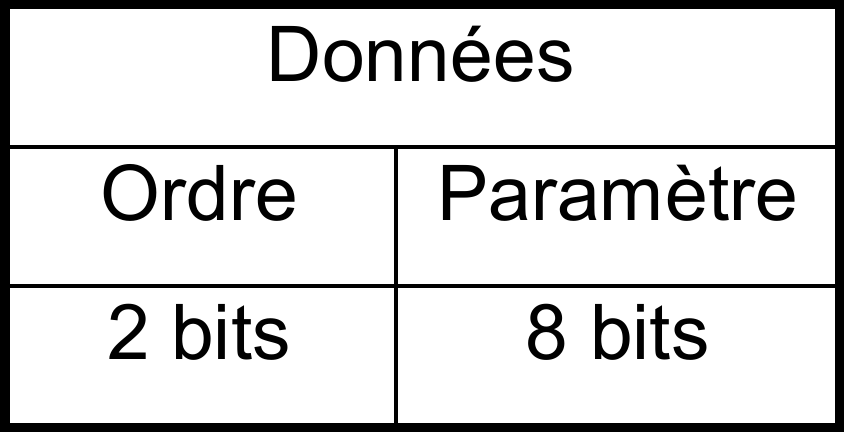
\includegraphics[width = 0.3\textwidth]{fskDetectorOutput.png}
  \caption{Format d'une trame à la sortie de \ilcode{fskDetector}.\label{fig:fskDetectorOutput}}
\end{figure}
C'est cette trame qui doit être divisée en deux trames de 8 bits. De plus, le récepteur doit pouvoir faire la différence entre les trames <<première partie>> et les trames <<deuxième partie>>, afin de pouvoir détecter certaines erreurs (partie manquante ou répétition) et pouvoir correctement reconstituer l'instruction reçue. Dans la suite, les les trames <<première partie>> seront notées T1 et les trames <<deuxième partie>> T2.

L'ordre ne peut prendre que les valeurs \ilcode{0b00}, \ilcode{0b10} ou \ilcode{0b01}. On choisit donc que la quatrième possibilité, \ilcode{0b11} constitue les deux premiers bits de T1 afin, de distinguer celle-ci de T2, dont les deux premiers bits sont l'ordre\footnote{Voir la section \ref{subsec:propReceptor} sur le récepteur propulsion pour voir pourquoi l'ordre est envoyé dans la deuxième trame.}. Les 8 bits de paramètre restants sont répartis entre T1 et T2. Il reste donc deux bits inutilisés dans chaque trame, qu'on met simplement à 0. Tout ceci est résumé dans la figure \ref{fig:fskToUART}.
\begin{figure}[htbp]
  \centering
  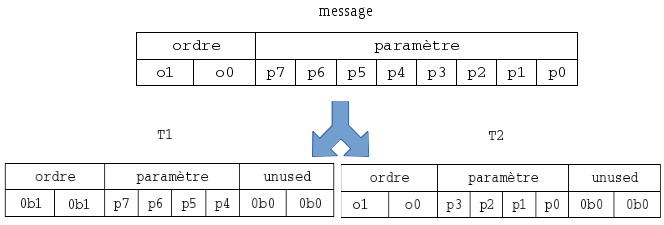
\includegraphics[width = 0.9\textwidth]{fskToUART.png}
  \caption{Division du message en deux trames UART.\label{fig:fskToUART}}
\end{figure}

A partir de ce format de trame, les émetteurs et récepteurs vont maintenant être construits en suivant l'émission d'une commande et en examinant tous les scénarios possibles.

\subsection{\'Emetteur communication}
L'entrée du bloc UART dans son entier est la fonction \ilcode{sendCommand(int newCommand)}. Comme des erreurs sont envisageables, le récepteur peut demander que la commande soit répétée. Pour cette raison, \ilcode{newCommand} est stockée de manière persistante avant d'être envoyée. Comme annoncé plus haut, les interruptions d'émissions sont utilisées pour envoyer les deux trames, et l'émetteur est une machine d'état séquentielle.

Lorsqu'une commande doit être envoyée, l'interruption d'émission est activée, et l'état de l'émetteur mis à zéro, ce qui correspond à aucune trame déjà envoyée. Ensuite, dans la routine d'émission, T1 ou T2 est construite selon l'état, puis envoyée, et l'état est incrémenté. Après l'envoi de T2, l'interruption est désactivée jusqu'à ce qu'une nouvelle commande doive être envoyée, et ainsi de suite. Ceci est exécuté par la routine d'émission.

Le récepteur propulsion est calqué sur cet émetteur et est présenté dans la section suivante.

\subsection{Récepteur propulsion\label{subsec:propReceptor}}
Le récepteur propulsion est donc lui aussi une machine d'état séquentielle à deux états.

A l'état 0, une T1 est attendue. Si c'est bien une T1 qui est reçue, alors l'état passe à 1 et \ilcode{p<7-4>} contenus dans la trame sont stockés. Sinon, il y a eu une erreur, l'état reste à 0 et l'UART propulsion demande que le message soit répété.

A l'état 1, une T2 est attendue. Si une T2 est reçue, alors le message a été entièrement reçu, l'état retourne à zéro et le récepteur retourne séparément \ilcode{o<1-0>} et \ilcode{p<7-0>} à partir de T2\footnote{On voit donc ici pourquoi il est plus intéressant d'envoyer l'ordre dans T2: cela permet de ne pas devoir le stocker à l'état 0.} et de \ilcode{p<7-4>} en mémoire. Sinon, il y a eu une erreur, l'état retourne aussi à zéro et l'UART propulsion demande que le message entier soit répété. Ceci est exécuté par la fonction \ilcode{handleReceived} qui appelle \ilcode{handleParam1} ou \ilcode{handleParam2} selon le type de trame reçue.

D'autres possibilités d'erreurs ont été vues plus haut: mauvaise parité (détecté par l'UART lui-même) ou mauvais formatage (détecté par l'UART ou le récepteur si LSB et LSB+1 d'une trame sont non nuls). Le mécanisme est systématiquement le même: l'état du récepteur retourne à zéro et la répétition du message est demandée par la fonction \ilcode{askRepeat}.

La demande de répétition du message est la seule chose que l'UART propulsion émet. L'émetteur propulsion est donc très simple. Il est présenté dans la section suivante.

\subsection{\'Emetteur propulsion}
L'émetteur propulsion n'envoie que des messages de une trame, et ce relativement rarement. On peut donc se contenter de vérifier (pour la forme) que l'on peut écrire dans la FIFO et d'y écrire la trame \ilcode{0x01} qui demande le renvoi de la commande. Il s'agit donc aussi de la seule trame que le récepteur communication peut doit gérer. Ce récepteur est donc lui aussi très simple. Il est présenté dans la section suivante.

\subsection{Récepteur communication}
Si l'UART communication reçoit une trame \ilcode{0x01}, il faut donc renvoyer la commande actuelle. Pour cela \ilcode{sendCommand(int newCommand)} est légèrement modifiée. Si \ilcode{newCommand} est \ilcode{0xFFFF} (pas un message valide), alors la commande gardée en mémoire n'est pas écrasée, et l'envoi déclenché ensuite renvoie donc la commande précédente. Ceci est fait par un simple test au début de la fonction \ilcode{sendCommand}

Le cas où la trame reçue côté communication n'est pas valide n'est pas géré: la transmission de la commande, s'il y avait bien une commande à transmettre au départ, est abandonnée. Ce cas ne s'est jamais présenté. Tous les scénarios possibles ont donc été examinés et le code présenté implémente donc une communication UART complète et parfaitement fonctionnelle. Ceci va être validé dans la section suivante.

Le traitement de l'ordre et du paramètre doit maintenant être abordé. Ce traitement est appelé dans la fonction \ilcode{handleParam2} du code source du récepteur propulsion par l'instruction \ilcode{interpretCommand(command, param);}, et va être présenté dans le chapitre suivant. La transmission de la commande entre les deux microcontrôleurs et l'interprétation de celle-ci seront validée en même temps à la fin du chapitre suivant.